\section{Methodology}\label{sec:method}

Our goal is to observe, for each MCP server, what its tools looked like when a user could first approve them and how they changed afterwards. We reconstruct this from public release histories: for every sampled version of a server we extract the tools it exposes, their descriptions, and the capabilities their code can reach, and we compare consecutive versions. Figure~\ref{fig:pipeline} summarizes the pipeline. All analysis is static; we never run a server.

\begin{figure*}[t]
\centering
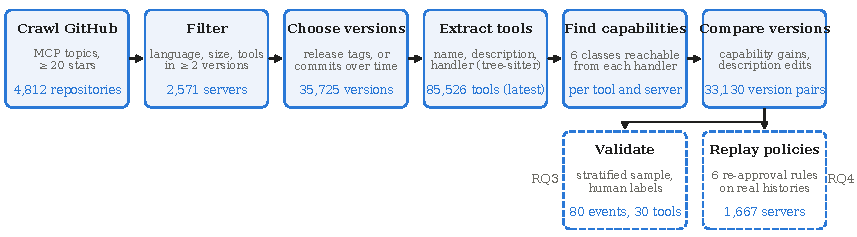
\includegraphics[width=\textwidth]{figures/fig_pipeline.pdf}
\caption{Measurement pipeline. Counts are for our study population; the two dashed steps use the version comparisons.}\label{fig:pipeline}
\end{figure*}

\subsection{Dataset}\label{sec:dataset}
We collected repositories from GitHub that carry the topics \texttt{mcp-server}, \texttt{model-context-protocol}, or \texttt{mcp-servers}, have at least 20 stars, and are neither forks nor archived. GitHub's search API returns at most 1,000 results per query, so we split each query into star ranges until every range fit under the cap. The crawl, run on November~2, 2026, returned 4,812 unique repositories.

We kept the 3,508 repositories whose primary language is Python, TypeScript, or JavaScript, the languages of the official MCP SDKs and of most servers. We then removed 248 repositories with more than 600 source files at their latest commit. These are monorepos and applications that embed an MCP server among many other components; in them, repository-wide capability signals say little about the server. Five repositories could not be cloned or timed out. Finally, we removed 684 repositories in which we found tools in fewer than two versions, since they offer nothing to compare. The remaining 2,571 servers form our study population (Table~\ref{tab:funnel}).

\begin{table}[t]
\centering\small
\caption{From crawl to study population.}\label{tab:funnel}
\begin{tabular}{lr}
\toprule
Step & Repositories \\
\midrule
Topic search, $\geq$20 stars, no forks or archives & 4,812 \\
Python, TypeScript, or JavaScript & 3,508 \\
\quad minus monorepos ($>$600 source files) & $-$248 \\
\quad minus clone failures and timeouts & $-$5 \\
\quad minus tools in fewer than two versions & $-$684 \\
\midrule
Study population & 2,571 \\
Sampled versions (median 8 per server) & 35,725 \\
\bottomrule
\end{tabular}
\end{table}

\subsection{Choosing versions}\label{sec:versions}
A user approves whatever version they install, so the natural unit is a release. For each repository we cloned the default branch and walked its first-parent history. When at least three release tags lie on that history, we used the tags, subsampling evenly to at most 40. Otherwise we took up to 12 commits spaced evenly in time between the first and the latest commit. We always included the latest commit. This yields 35,725 versions, a median of 8 per server. Sampling means we see a lower bound on how often servers change: two releases we skip may hide a change that was introduced and later reverted.

\subsection{Extracting tools}\label{sec:tools}
At each version we parsed every source file with tree-sitter, skipping tests, examples, documentation, vendored code, build output, and build or test configuration files. We recognize the registration patterns of the official Python and TypeScript SDKs and of common frameworks: decorators such as \texttt{@mcp.tool()}, imperative calls such as \texttt{server.add\_tool(...)}, \texttt{server.tool(...)} and \texttt{registerTool(...)}, \texttt{Tool(name=..., description=...)} objects, and object or dictionary literals that carry a name, a description, and an input schema or handler. For each tool we record its name, its description as the client would receive it, and its handler. We resolve descriptions built from string concatenation, module constants, or docstrings; descriptions computed at run time are marked as dynamic and excluded from description comparisons.

\subsection{Detecting capabilities}\label{sec:caps}
We track six capability classes that matter for approval: running shell commands or other programs, evaluating dynamically constructed code, writing or deleting files, reading files, reading environment variables or credential stores, and network access. Each class is a set of API patterns, for example \texttt{subprocess.*} and \texttt{child\_process} for shell execution, or \texttt{process.env} and \texttt{os.environ} for environment access. We also record every external hostname that appears in a URL literal.

A capability belongs to a tool if the tool's handler can reach it. We start at the handler and follow calls to functions defined in the same repository, up to four calls deep. Name-based call resolution is error-prone, and our first version of the extractor was wrong in ways our validation exposed (Section~\ref{sec:rq3}), so we apply four rules. We match patterns only in code, not inside comments or long string literals: a tool that returns a shell command as text does not itself run a shell. We do not treat imports of constant module names as dynamic code. We follow only bare calls and calls on \texttt{self}, \texttt{this}, or \texttt{cls}; a call such as \texttt{db.execute(...)} has a target we cannot know statically. And we never resolve generic names such as \texttt{run} or \texttt{execute}; when a name has several definitions, we take the one in the tool's own file or package, and otherwise none. For each capability we record whether it appears in the handler itself or which helper introduces it.

Tool-level attribution can miss capabilities reached through dynamic dispatch or third-party libraries. We therefore also record server-level capabilities: the classes found anywhere in the server's source.

\subsection{Comparing versions}\label{sec:diff}
For each server we start at the first version that exposes tools and compare each version with the next. A tool keeps its identity across versions by name. For every tool present in both versions we record capability gains and description changes. We also record new tools, new server-level capabilities, new external hostnames, and new declared dependencies. Versions in which we extract no tools are skipped rather than treated as removing every tool.

We call a capability gain \emph{silent} if the tool's description is byte-identical before and after. A server-level gain is silent if, in the same step, no tool description changed, no tool was added, and the README did not change. When the description did change, we call the gain \emph{disclosed} if the new text, but not the old, matches a keyword pattern for the gained class (for running commands, words such as \emph{shell}, \emph{command}, or \emph{execute}), and \emph{undisclosed} otherwise. The match is deliberately permissive, so it overestimates disclosure.

\subsection{Validation}\label{sec:validation}
We validate the two steps a reader has to trust: that the tools we extract are real, and that the changes we report happened.

\paragraph{Tools}
An author opened the source of 30 randomly sampled extracted tools and checked whether each is registered as an MCP tool and whether the extracted description is the text a client would receive.

\paragraph{Changes}
We drew a seeded, stratified sample of 200 events from five strata: silent high-risk gains found in a tool's own handler, silent high-risk gains found through a helper, other capability gains, silent server-level gains, and description changes that matched instruction-like text. Taking at most one event per server per stratum keeps prolific repositories from dominating. For each sampled event we prepared a \emph{code map} with a large language model instructed to report facts and no judgments: the server's purpose from its README, the tool's registration and description at both versions, the call path from the handler to each capability, what changed between the versions, and whether the flagged capability is reachable from the tool. Every statement in a map carries a file and line reference, so it can be checked against the source.

One author labeled the first 16 events of each stratum in a seeded random order, 80 in total, reading the map and the source code. No model proposed labels. Labels follow a fixed decision procedure. A change is an \emph{extraction error} if the flagged capability is not reachable from the tool (the code sits in tests, build scripts, a command-line entry point, or another tool, or the extractor matched the wrong function), or if the tool could already do the same in the earlier version. Otherwise it is \emph{security-relevant} if it gives the tool new access to credentials, lets the model's input shape a command, code, or file path, writes outside the server's own data, sends data to a new destination, or contradicts the description; and \emph{benign} if it is routine for the tool's purpose, such as reading a non-secret setting or writing the server's own cache. For description changes, the label is an extraction error if the text did not really change, security-relevant if the new text hides content or steers the model toward unrelated data or tools, and benign otherwise. An annotator may answer \emph{unsure}.

We report precision per stratum with 95\% Wilson intervals, and the agreement (Cohen's $\kappa$) between the human label and the map's reachability verdict, reduced to whether the flagged change is real. Labels received a second pass against the written definitions; we report agreement for the first pass (Section~\ref{sec:rq3}).

\subsection{Limitations of the method}\label{sec:limits}
Static analysis shows that a code path exists, not that it runs. We see only capabilities expressed through the APIs we model; code that hides in dependencies, downloads behavior at run time, or uses unusual APIs escapes us, so our capability counts are lower bounds for a determined adversary. We study git histories, while users install packages from npm or PyPI that may differ from the repository. Our population favors popular, open-source servers in three languages. Sampling releases understates the number of changes. Our labels come from a single annotator, so we cannot report agreement between humans, and because we label only flagged events we measure precision but not recall. We return to these limits in Section~\ref{sec:discussion}.
